\documentclass[12pt,a4paper]{article}

% Encodage et polices
\usepackage[utf8]{inputenc}
\usepackage[T1]{fontenc}

% Packages mathématiques et symboles
\usepackage{amsmath,amssymb,amsfonts}

% Gestion de la mise en page
\usepackage{geometry}
\geometry{margin=2.5cm}

% Interligne
\usepackage{setspace}
\onehalfspacing

% Hyperliens et images
\usepackage{hyperref}
\usepackage{graphicx}

\title{Analyse Statistique d'un Corpus Poétique}
\author{José Manuel Rodríguez Caballero}
\date{\today}

\begin{document}
	
	\maketitle
	\tableofcontents
	
	%============================================================
	\section{Description du Jeu de Données}
	%============================================================
	
	Le corpus étudié se compose de poèmes provenant de différents auteurs, 
	dont certains sont reconnus comme suicidaires. Plusieurs étapes de nettoyage 
	ont abouti à un ensemble final de données, organisé selon \textbf{quatre niveaux} :
	
	\begin{enumerate}
		\item \textbf{Cas-Témoin} : identifiés par \texttt{pair\_id} 
		(chaque poète suicidaire est apparié à un poète non suicidaire).
		\item \textbf{Poète} : chaque auteur est décrit par diverses informations biographiques 
		(dates, pays, orientation, etc.) et par un indicateur \texttt{suicidal}.
		\item \textbf{Poème} : chaque recueil de vers possède une période (\texttt{Early}, \texttt{Middle}, 
		\texttt{Later}), un titre, etc.
		\item \textbf{Vers} : unité de base pour la mesure des émotions (colère, joie, tristesse, etc.).
	\end{enumerate}
	
	\subsection{Étapes de constitution}
	\paragraph{\texttt{raw\_data.csv}}  
	Fichier de départ (42 lignes), chaque ligne représentant un poème, 
	avec des métadonnées (dates, pays, lien source, etc.).
	
	\paragraph{\texttt{clean\_data\_1.csv}}  
	Fichier intermédiaire où chaque vers est placé sur une ligne 
	(2931 lignes au total). Les informations du poète sont dupliquées 
	pour chaque vers du même auteur.
	
	\paragraph{\texttt{clean\_data\_2.csv}}  
	Fichier final à granularité identique (1 vers par ligne), 
	où le texte du vers est remplacé par des scores émotionnels 
	(\texttt{anger}, \texttt{joy}, \texttt{sadness}, etc.).
	
	\subsection{Données manquantes}
	\begin{itemize}
		\item Les 10 scores d’émotions ne comportent aucune valeur manquante.
		\item Au niveau Poète, la variable \texttt{heterosexual} contient 2 valeurs manquantes (\texttt{NA}).
		\item Les autres champs (dates, pays, etc.) sont complets. 
	\end{itemize}
	Le nombre de valeurs manquantes étant très faible, on considère que cela n’entrave pas l’analyse.
	
	%============================================================
	\section{Présentation des Variables}
	%============================================================
	
	\subsection{Niveau Cas-Témoin}
	\begin{itemize}
		\item \texttt{pair\_id} : identifiant de la paire (poète suicidaire vs. poète témoin).
	\end{itemize}
	
	\subsection{Niveau Poète}
	\begin{itemize}
		\item \texttt{poet} : nom de l’auteur (14 distincts).
		\item \texttt{suicidal} : \texttt{TRUE} ou \texttt{FALSE} (7 de chaque).
		\item \texttt{sex} : \texttt{Male} / \texttt{Female}.
		\item \texttt{heterosexual} : \texttt{TRUE} / \texttt{FALSE} / \texttt{NA}.
		\item \texttt{date\_of\_birth}, \texttt{date\_of\_death} : dates.
		\item \texttt{country\_of\_birth} : pays.
	\end{itemize}
	
	\subsection{Niveau Poème}
	\begin{itemize}
		\item \texttt{period} : \texttt{Early}, \texttt{Middle} ou \texttt{Later}.
		\item \texttt{poem\_title} : titre du poème.
	\end{itemize}
	
	\subsection{Niveau Vers}
	\begin{itemize}
		\item \texttt{anger}, \texttt{anticipation}, \texttt{disgust}, \texttt{fear}, 
		\texttt{joy}, \texttt{sadness}, \texttt{surprise}, \texttt{trust}, 
		\texttt{negative}, \texttt{positive} : scores d’émotions.
		\item Chacune de ces variables est un compteur ou une pondération de mots 
		associés à l’émotion concernée.
		\item Nombre d'observations : 2931
	\end{itemize}
	

	
%============================================================
\section{Analyse en Composantes Principales (ACP)}
%============================================================

\subsection{Principe et Préparation}
L'objectif est de résumer les différences émotionnelles entre poètes à l'aide 
d'une \textbf{analyse en composantes principales (ACP)}. 
Pour chaque poète, on calcule la moyenne de ses scores d'émotion 
(\texttt{anger}, \texttt{joy}, \texttt{negative}, etc.), 
obtenant ainsi un vecteur dans $\mathbb{R}^{10}$. 
La matrice finale, de taille $14 \times 10$, est ensuite ``centrée-réduite'', 
de sorte que chaque variable ait une moyenne nulle et un écart-type unitaire. 

\subsection{Éboulis des Valeurs Propres (Scree Plot)}
La Figure~\ref{fig:scree_plot} présente l'éboulis des valeurs propres. 
Chaque barre correspond à la proportion de variance expliquée par une composante principale. 
Ici, on constate que les deux premières composantes 
expliquent déjà plus de 75\,\% de la variance cumulée. 
Cela motive l'examen plus approfondi des axes PC1 et PC2.

\begin{figure}[htbp]
	\centering
	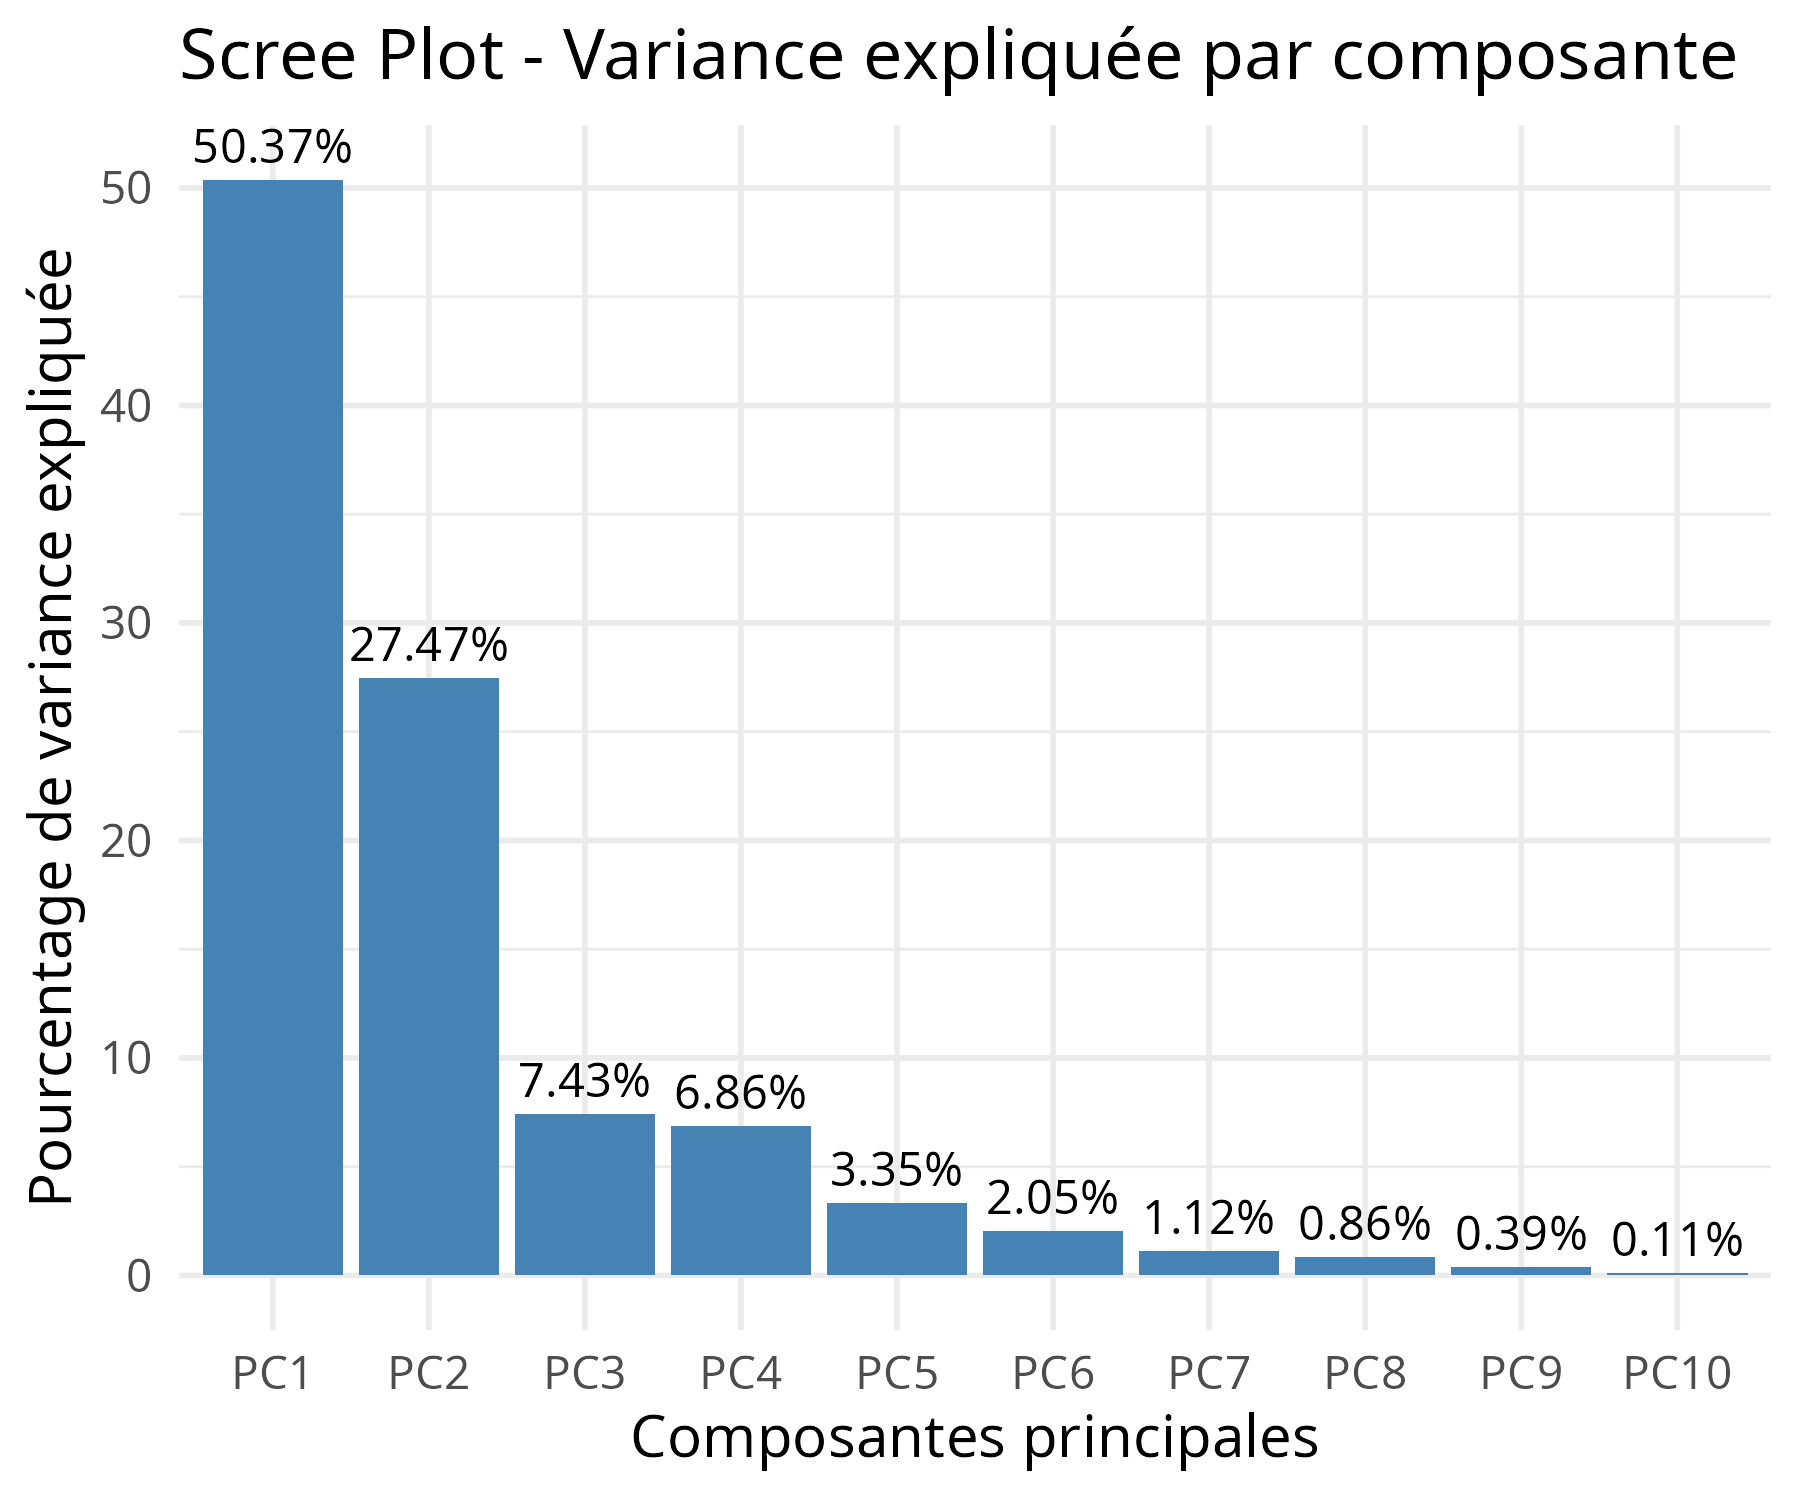
\includegraphics[width=0.65\textwidth]{01_scree_plot.png}
	\caption{Éboulis des valeurs propres : part de la variance expliquée par chaque composante (PC1 à PC10).}
	\label{fig:scree_plot}
\end{figure}

\subsection{Projection des Poètes (PC1, PC2)}
Dans la Figure~\ref{fig:acp_ind}, on projette les poètes (individus) 
dans le plan formé par les deux premières composantes principales. 
Les points sont colorés en fonction du statut \texttt{suicidal} 
(\texttt{TRUE} ou \texttt{FALSE}). 

\begin{figure}[htbp]
	\centering
	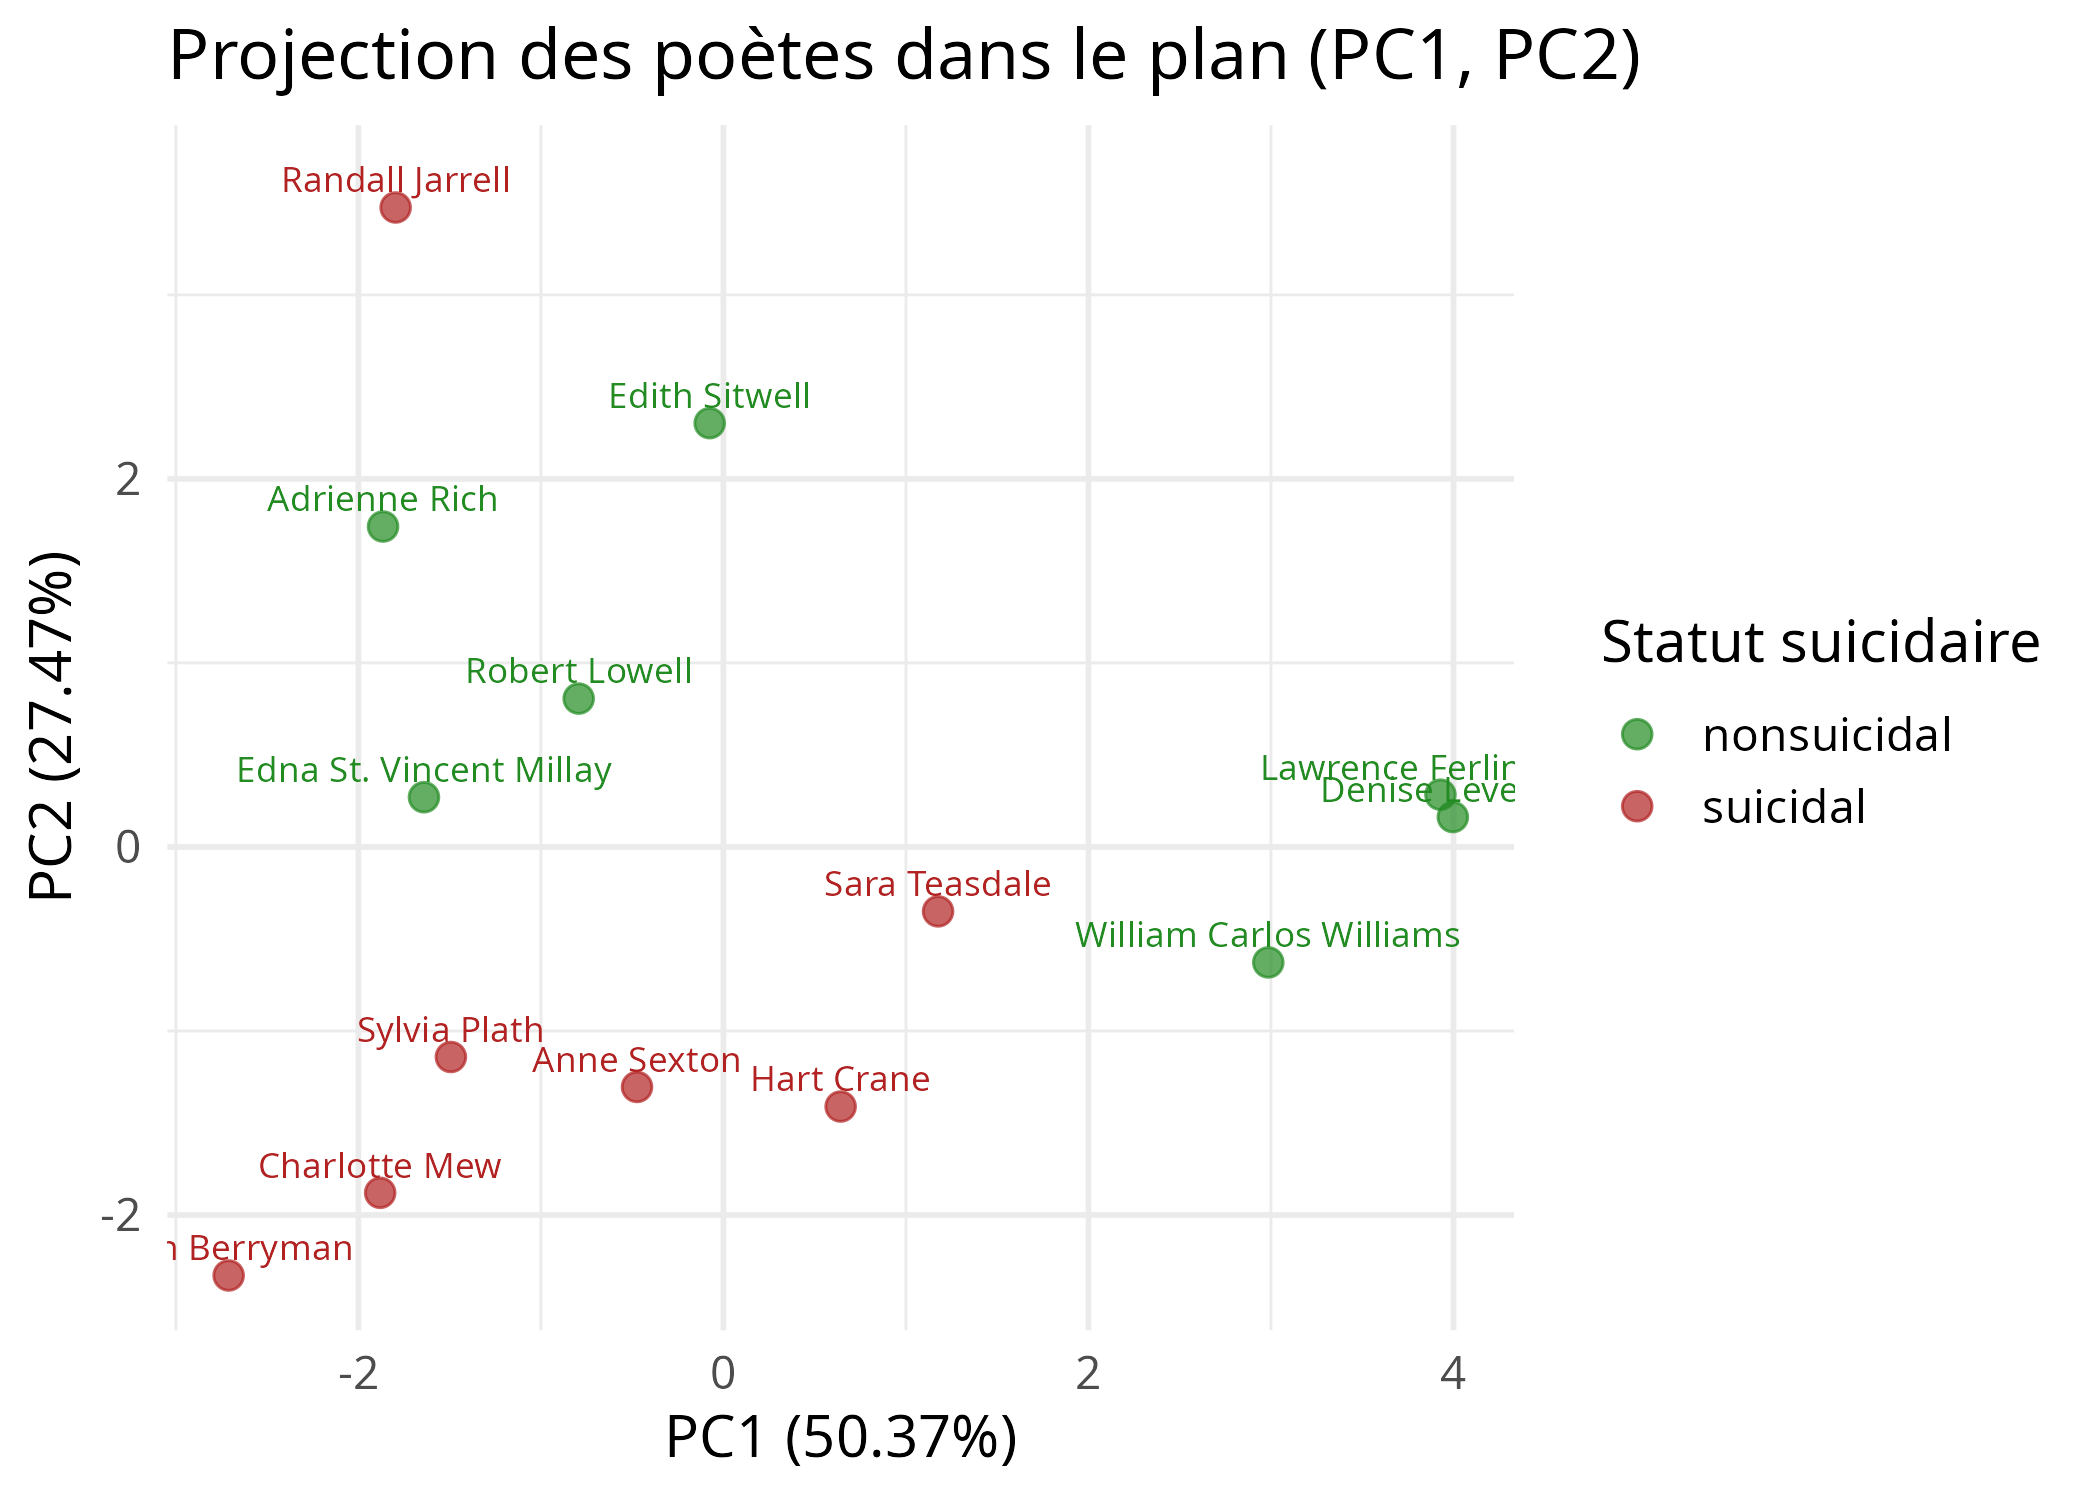
\includegraphics[width=1\textwidth]{02_individuals_PC1_PC2.png}
	\caption{Projection des poètes sur les deux premières composantes principales (PC1 et PC2).}
	\label{fig:acp_ind}
\end{figure}

Même si l'on observe une dispersion relativement importante, 
on peut investiguer si les poètes suicidaires se situent dans une zone distincte. 
Nous discutons plus loin (Section~\ref{subsec:test_pc}) 
de la comparaison statistique des scores de PC1 et PC2 selon le statut suicidaire.

\subsection{Visualisation des Variables (Biplot et Cercle de Corrélations)}
\paragraph{Biplot.}
La Figure~\ref{fig:pca_biplot} superpose la projection des individus (poètes) 
et des variables (émotions) dans le même plan. Les flèches indiquent 
la direction d'accroissement d'une émotion particulière, 
et leur longueur traduit l'importance de la représentation sur PC1--PC2. 
Un poète situé dans la même direction qu'une flèche 
présente une valeur élevée pour cette émotion (par rapport aux autres).

\begin{figure}[htbp]
	\centering
	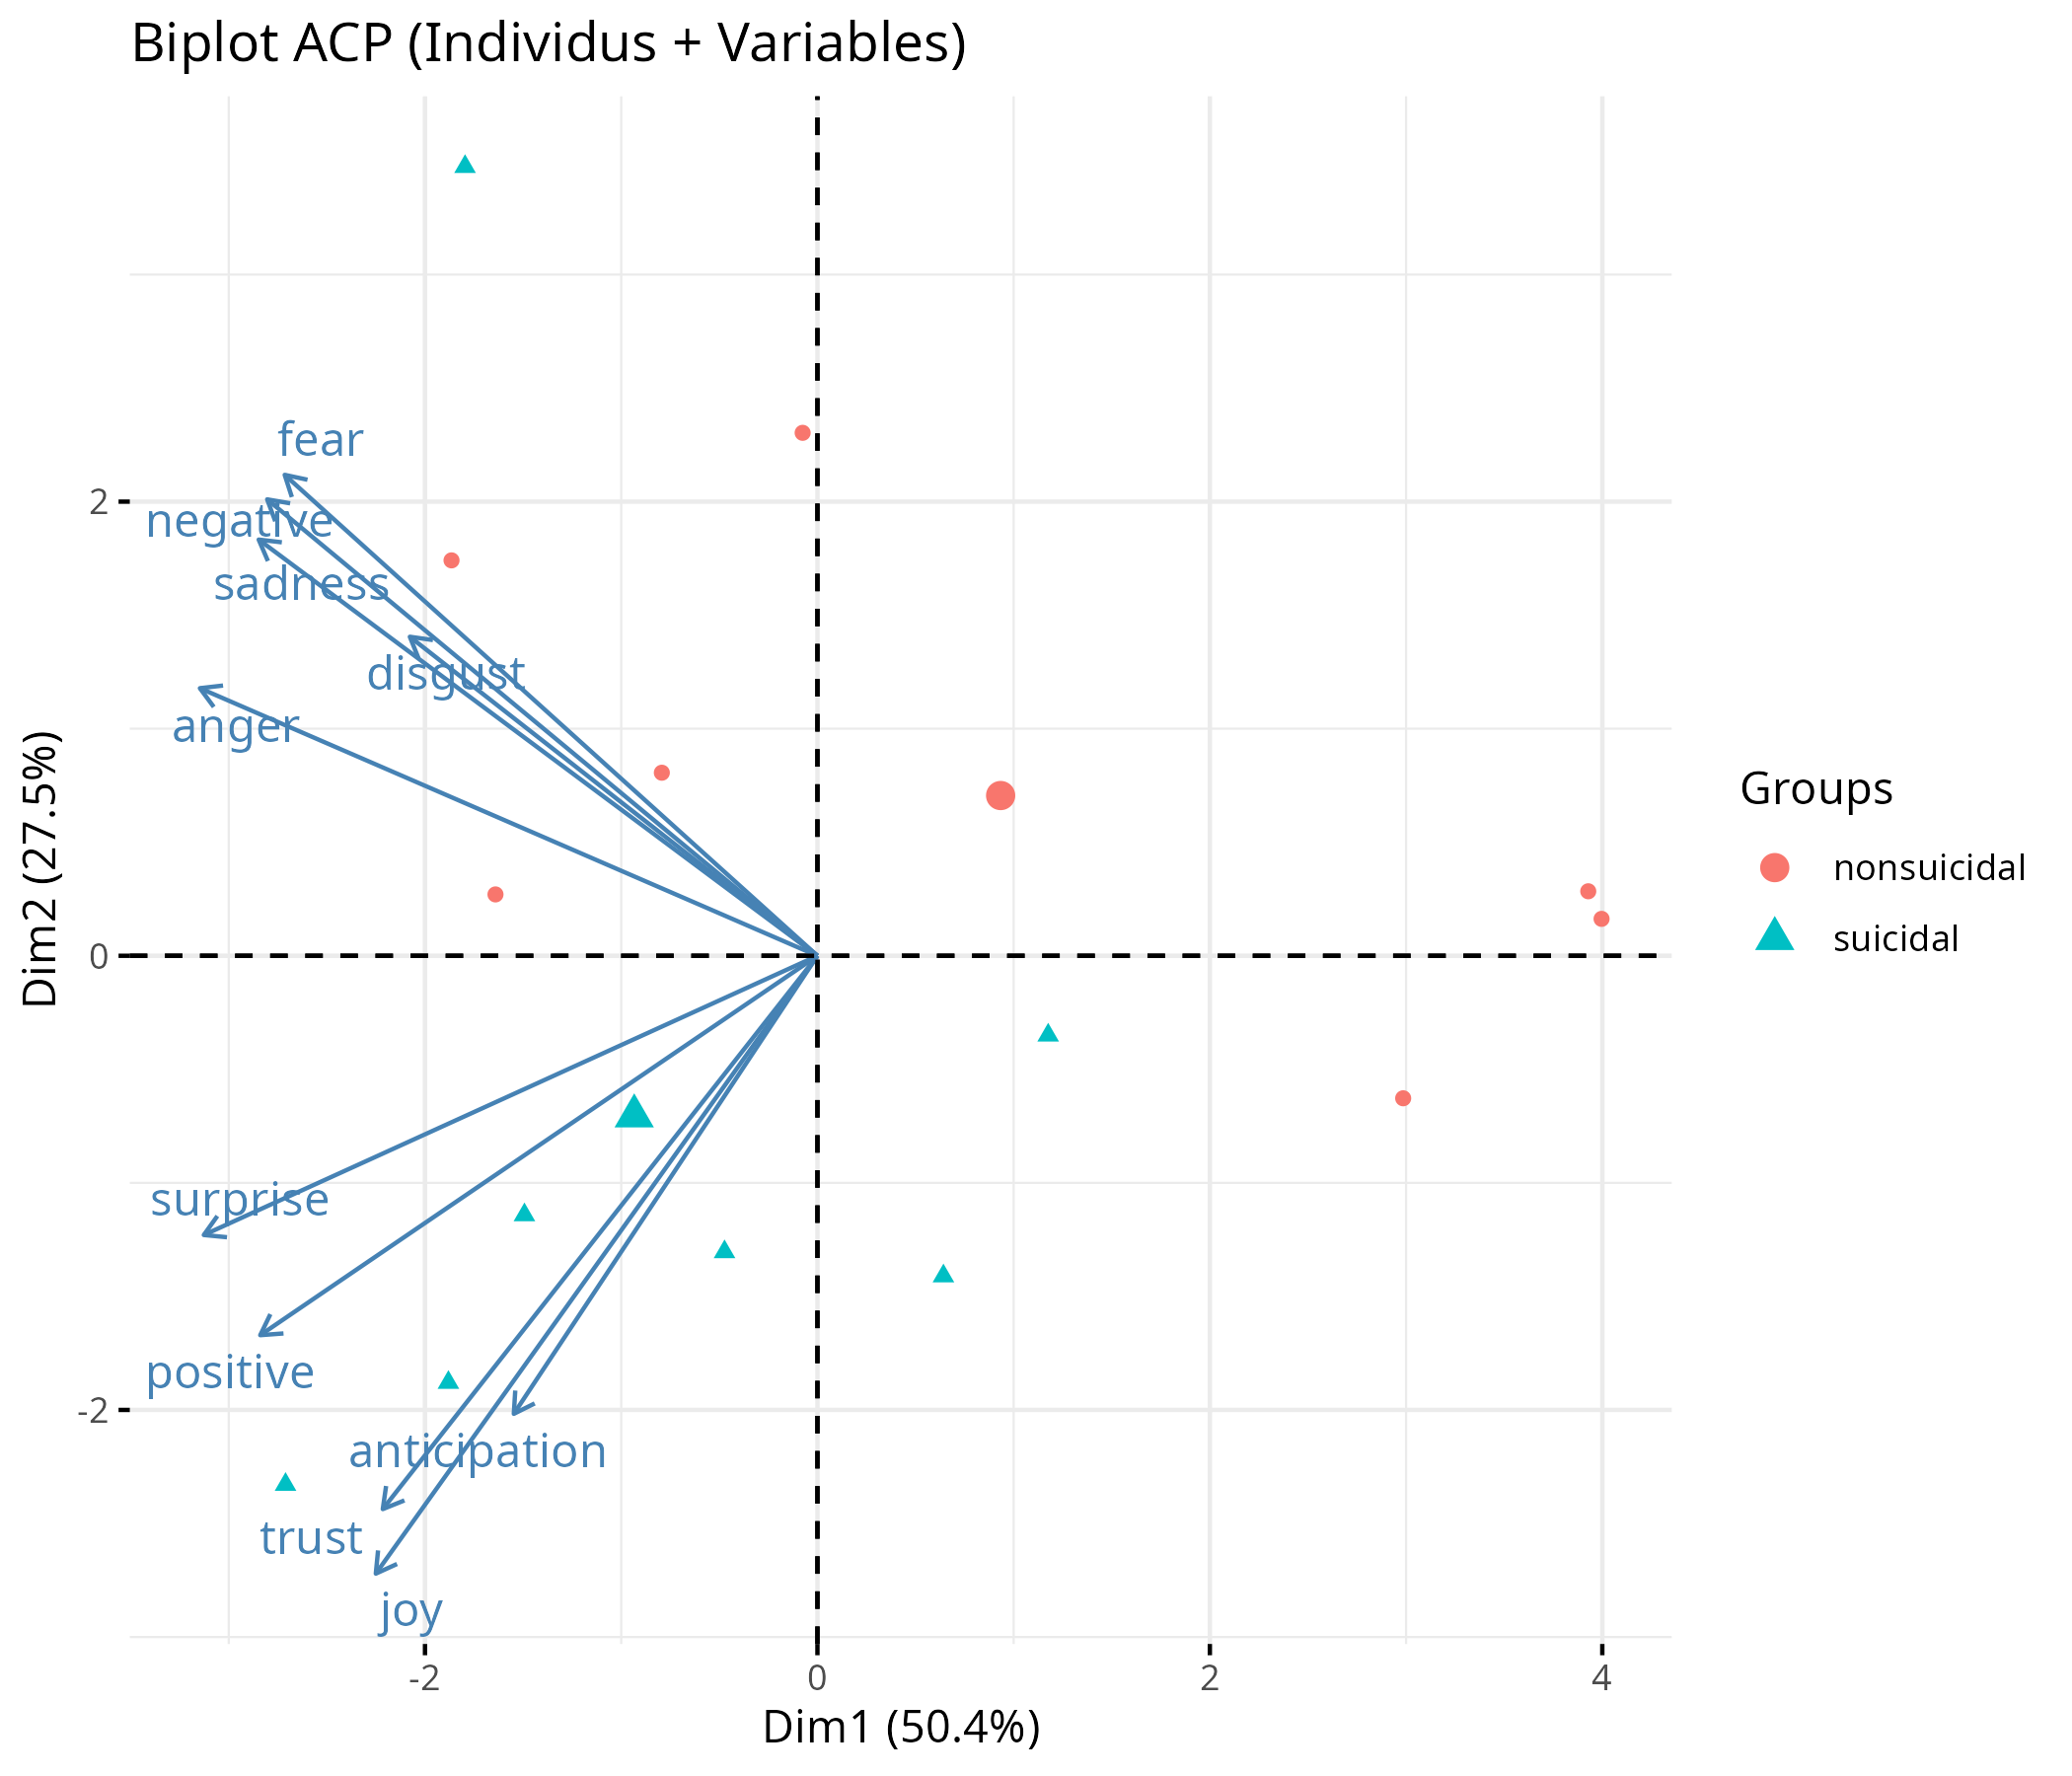
\includegraphics[width=0.7\textwidth]{03_pca_biplot.png}
	\caption{Biplot ACP : individus et variables (émotions) dans le plan (PC1, PC2).}
	\label{fig:pca_biplot}
\end{figure}

\paragraph{Cercle des Corrélations.}
La Figure~\ref{fig:pca_vars} illustre uniquement les émotions (variables) 
et leurs corrélations dans l'espace des deux premières composantes. 
Deux variables dont les vecteurs forment un angle faible 
sont positivement corrélées (et inversement pour un angle proche de 180°). 
Plus le vecteur est long, plus la variable est bien représentée par PC1--PC2.

\begin{figure}[htbp]
	\centering
	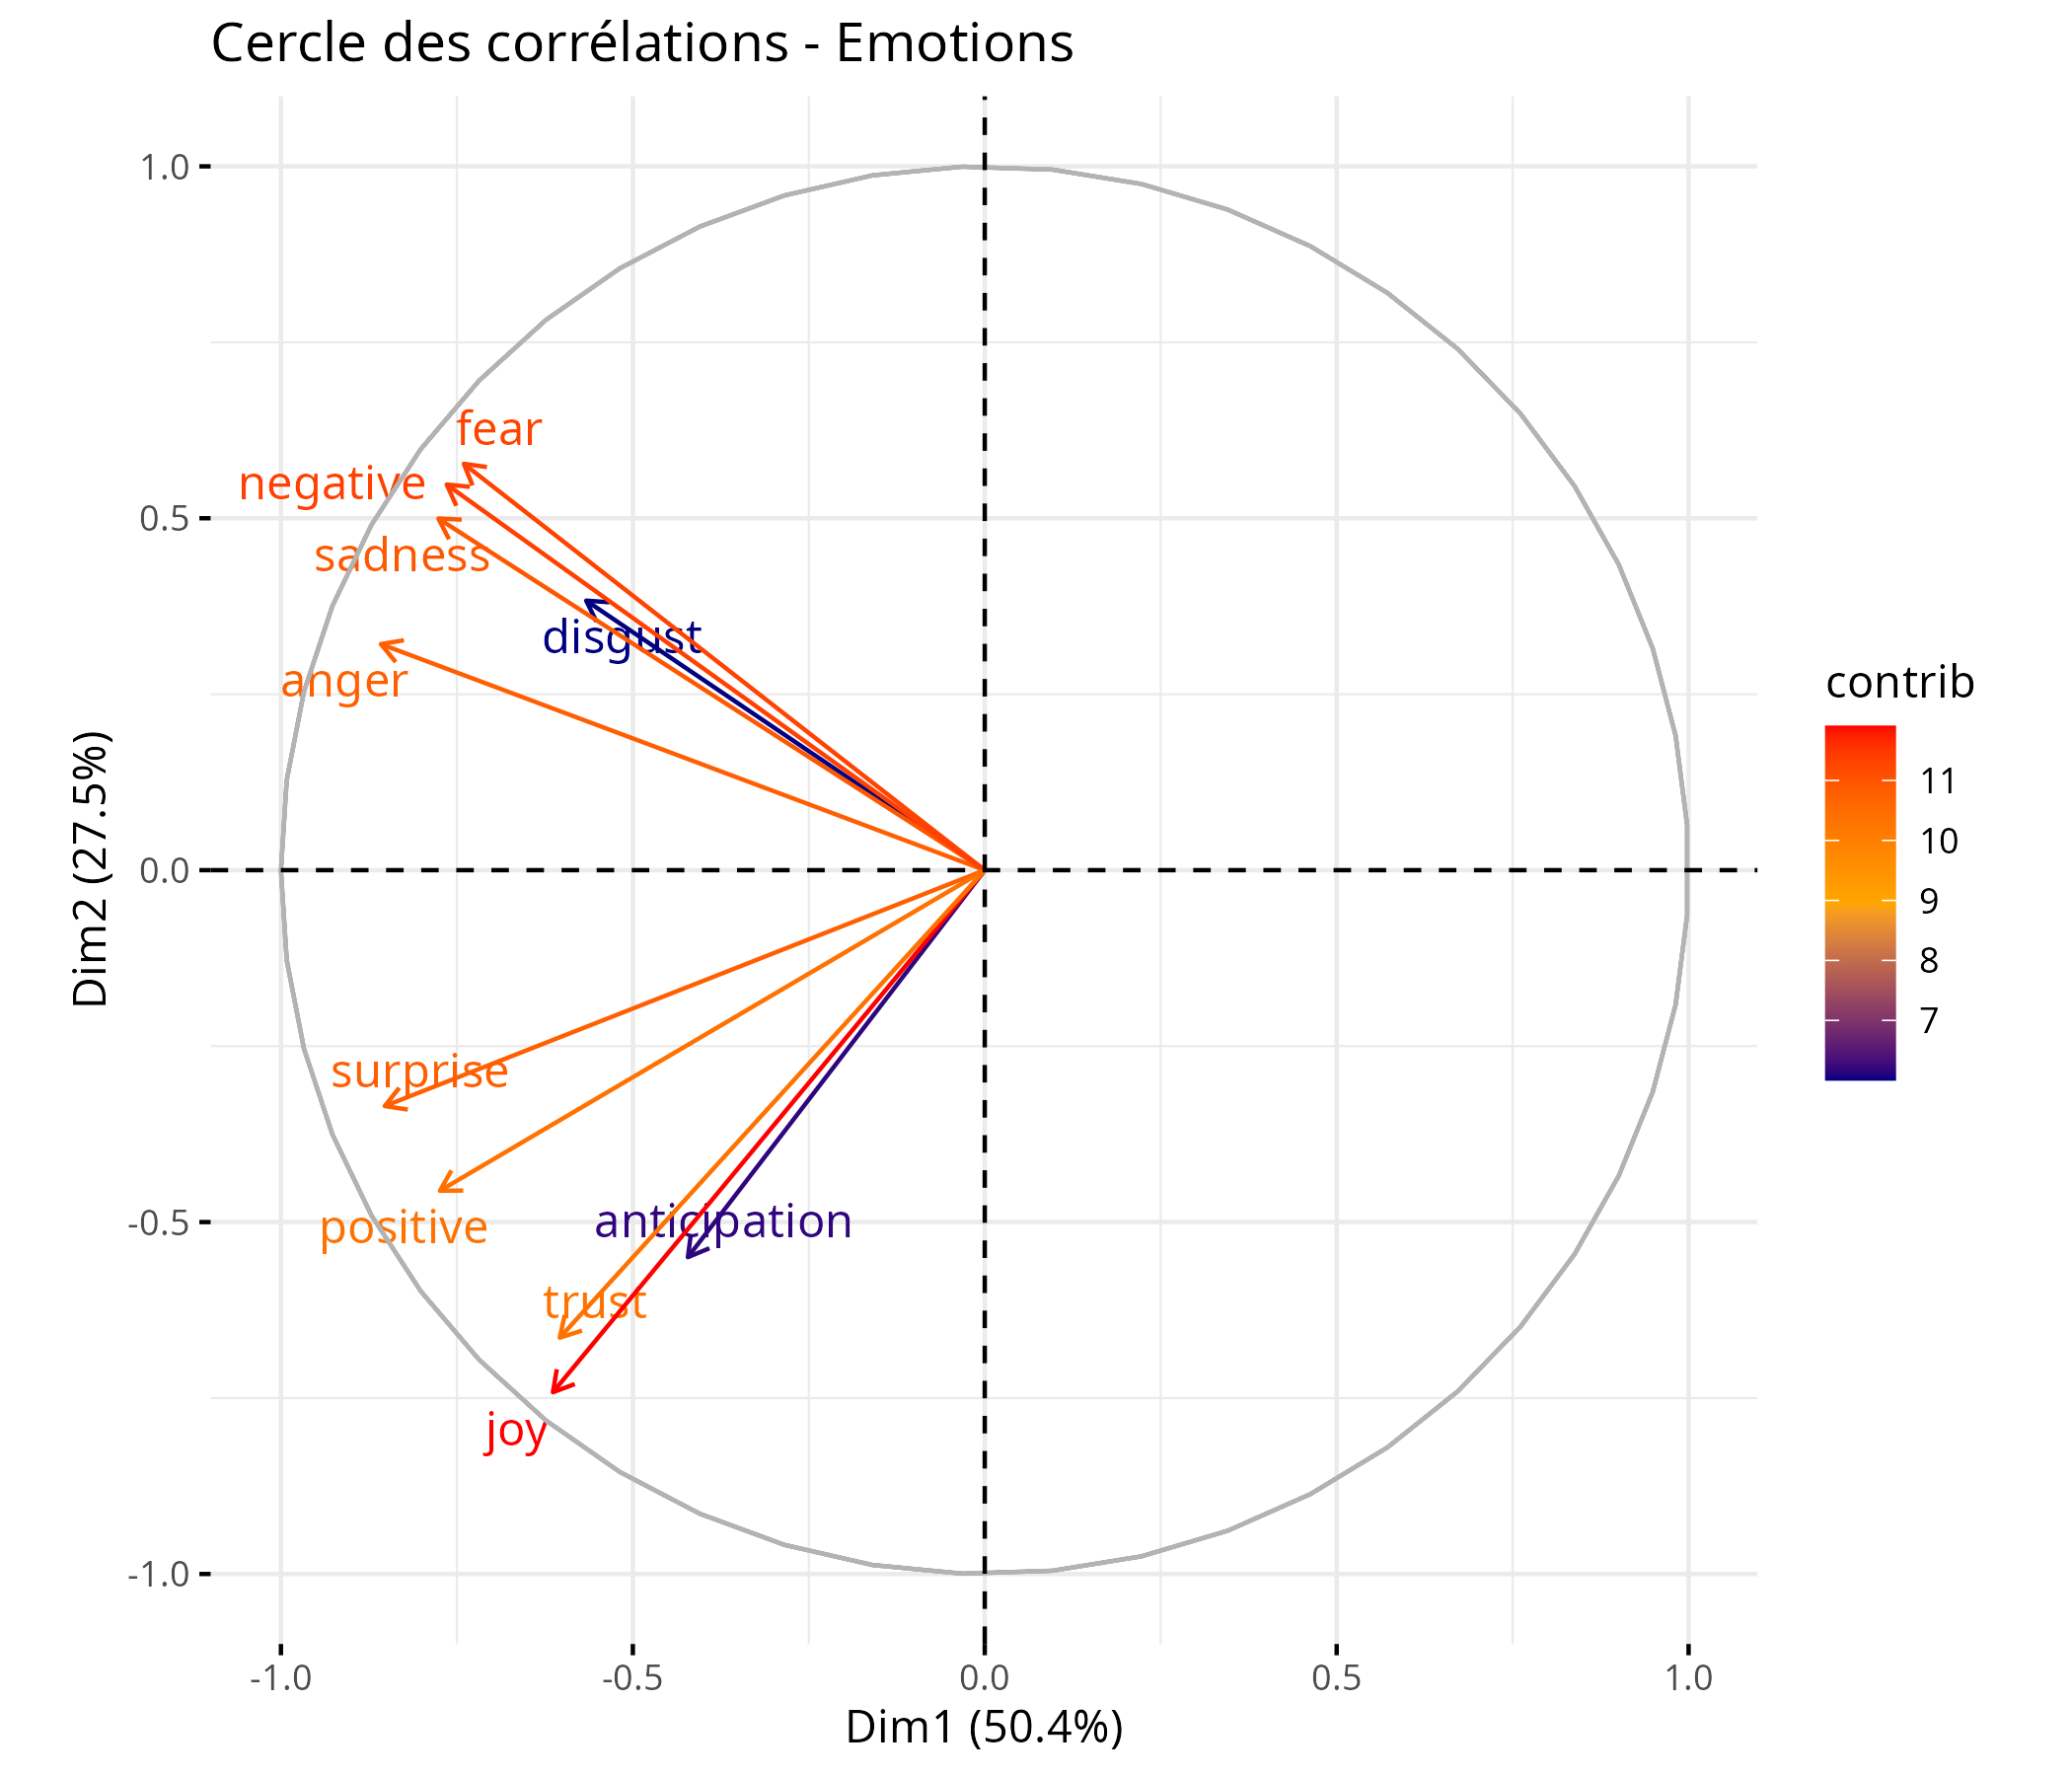
\includegraphics[width=0.6\textwidth]{04_correlations_circle.png}
	\caption{Cercle des corrélations : variables émotionnelles projetées sur PC1 et PC2.}
	\label{fig:pca_vars}
\end{figure}

\subsection{Comparaison Statistique des Scores sur PC1 et PC2}
\label{subsec:test_pc}
Pour évaluer si la position des poètes sur les deux premiers axes 
diffère significativement selon le statut \texttt{suicidal}, 
on compare ci-après les distributions de PC1 et PC2 par groupe.

\begin{figure}[htbp]
	\centering
	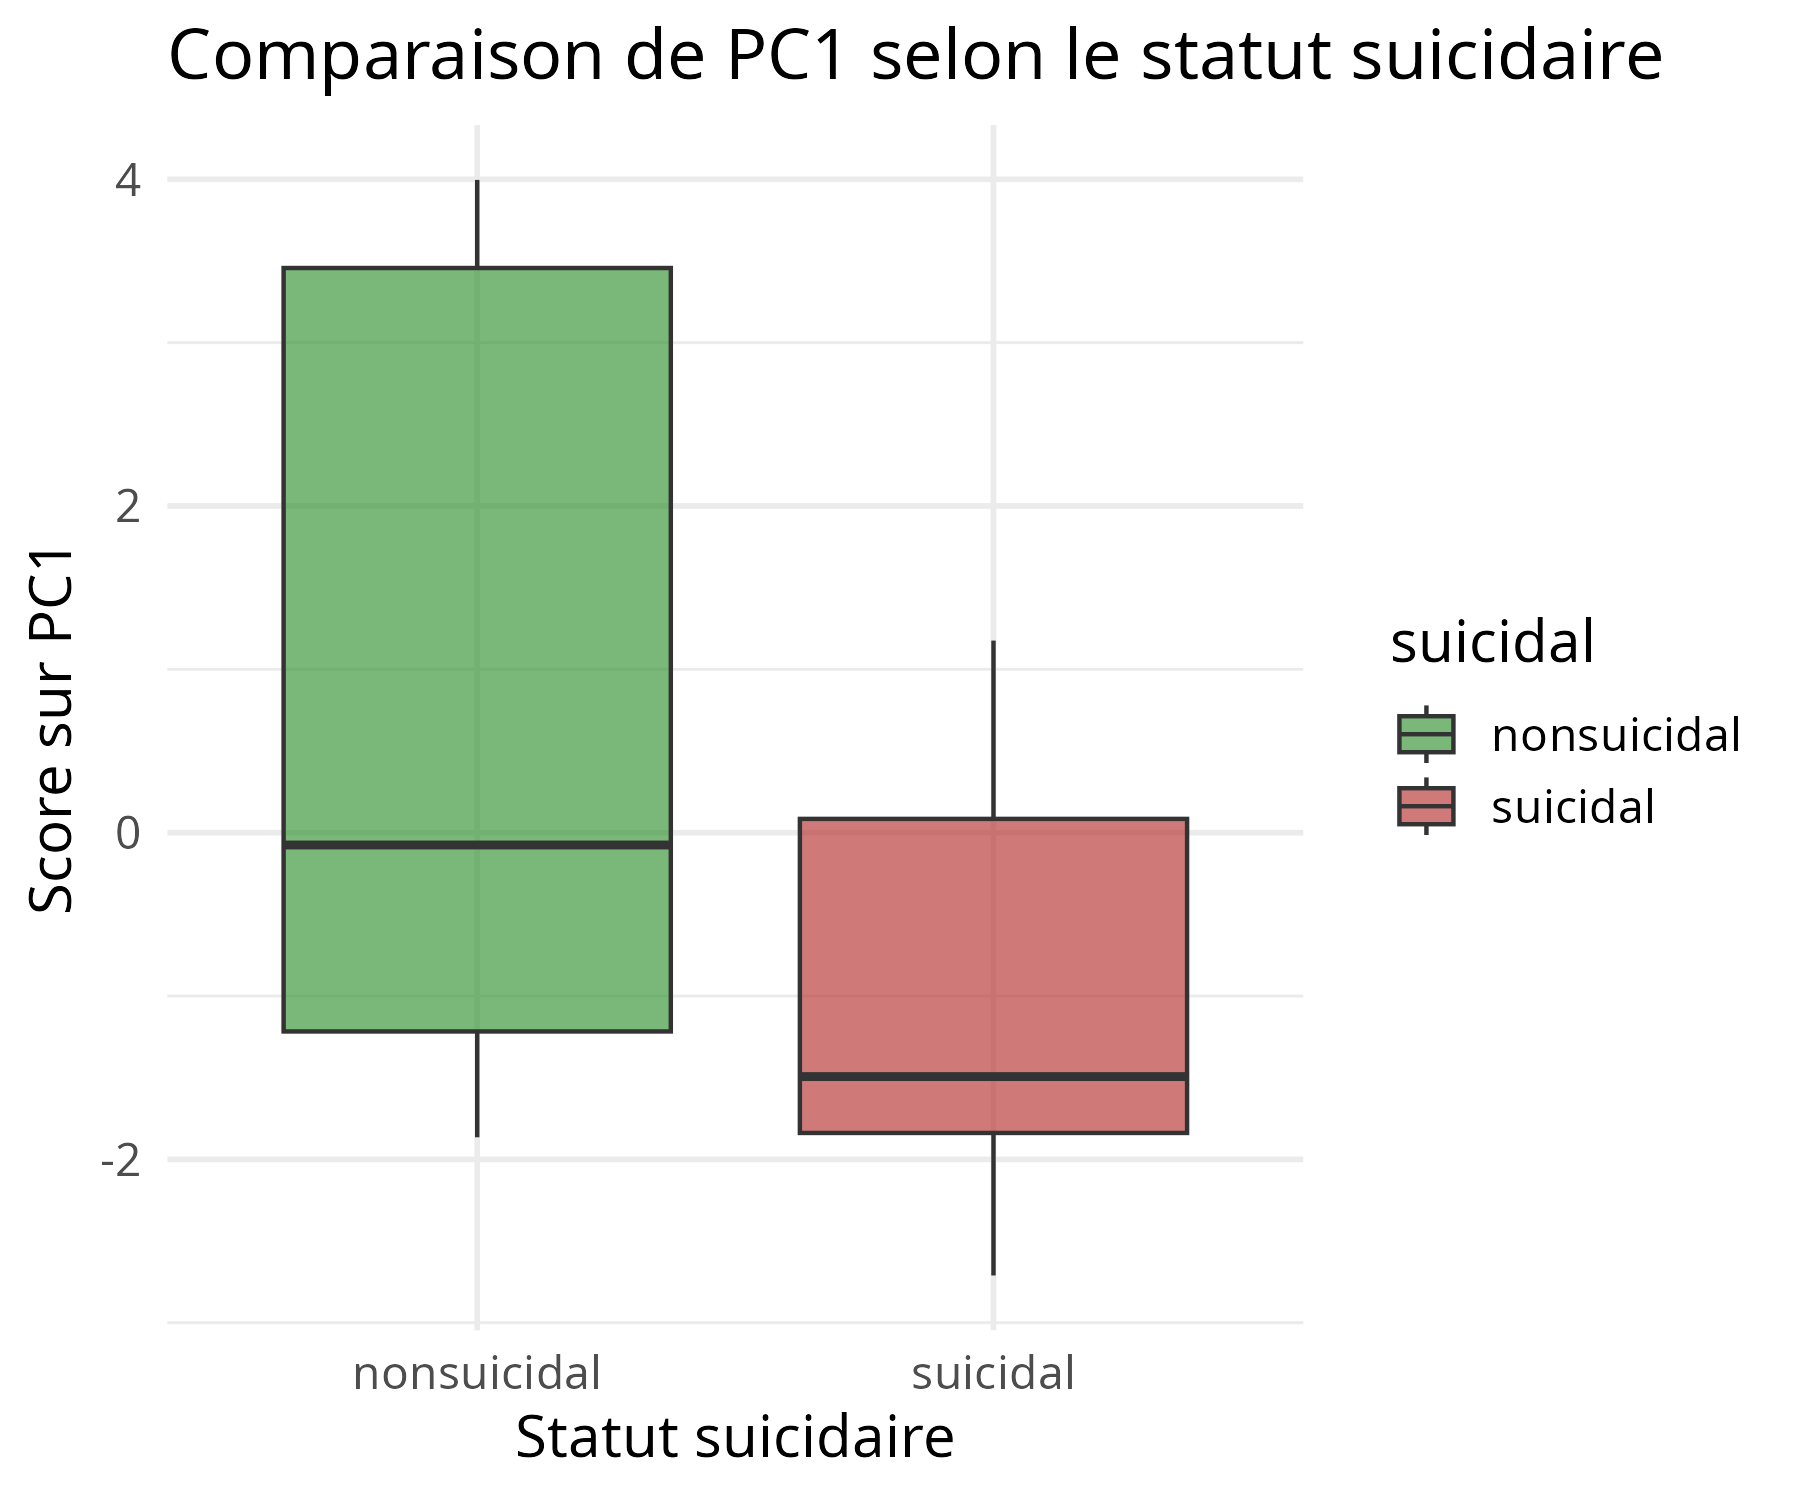
\includegraphics[width=0.49\textwidth]{05_boxplot_PC1.png}
	\hfill
	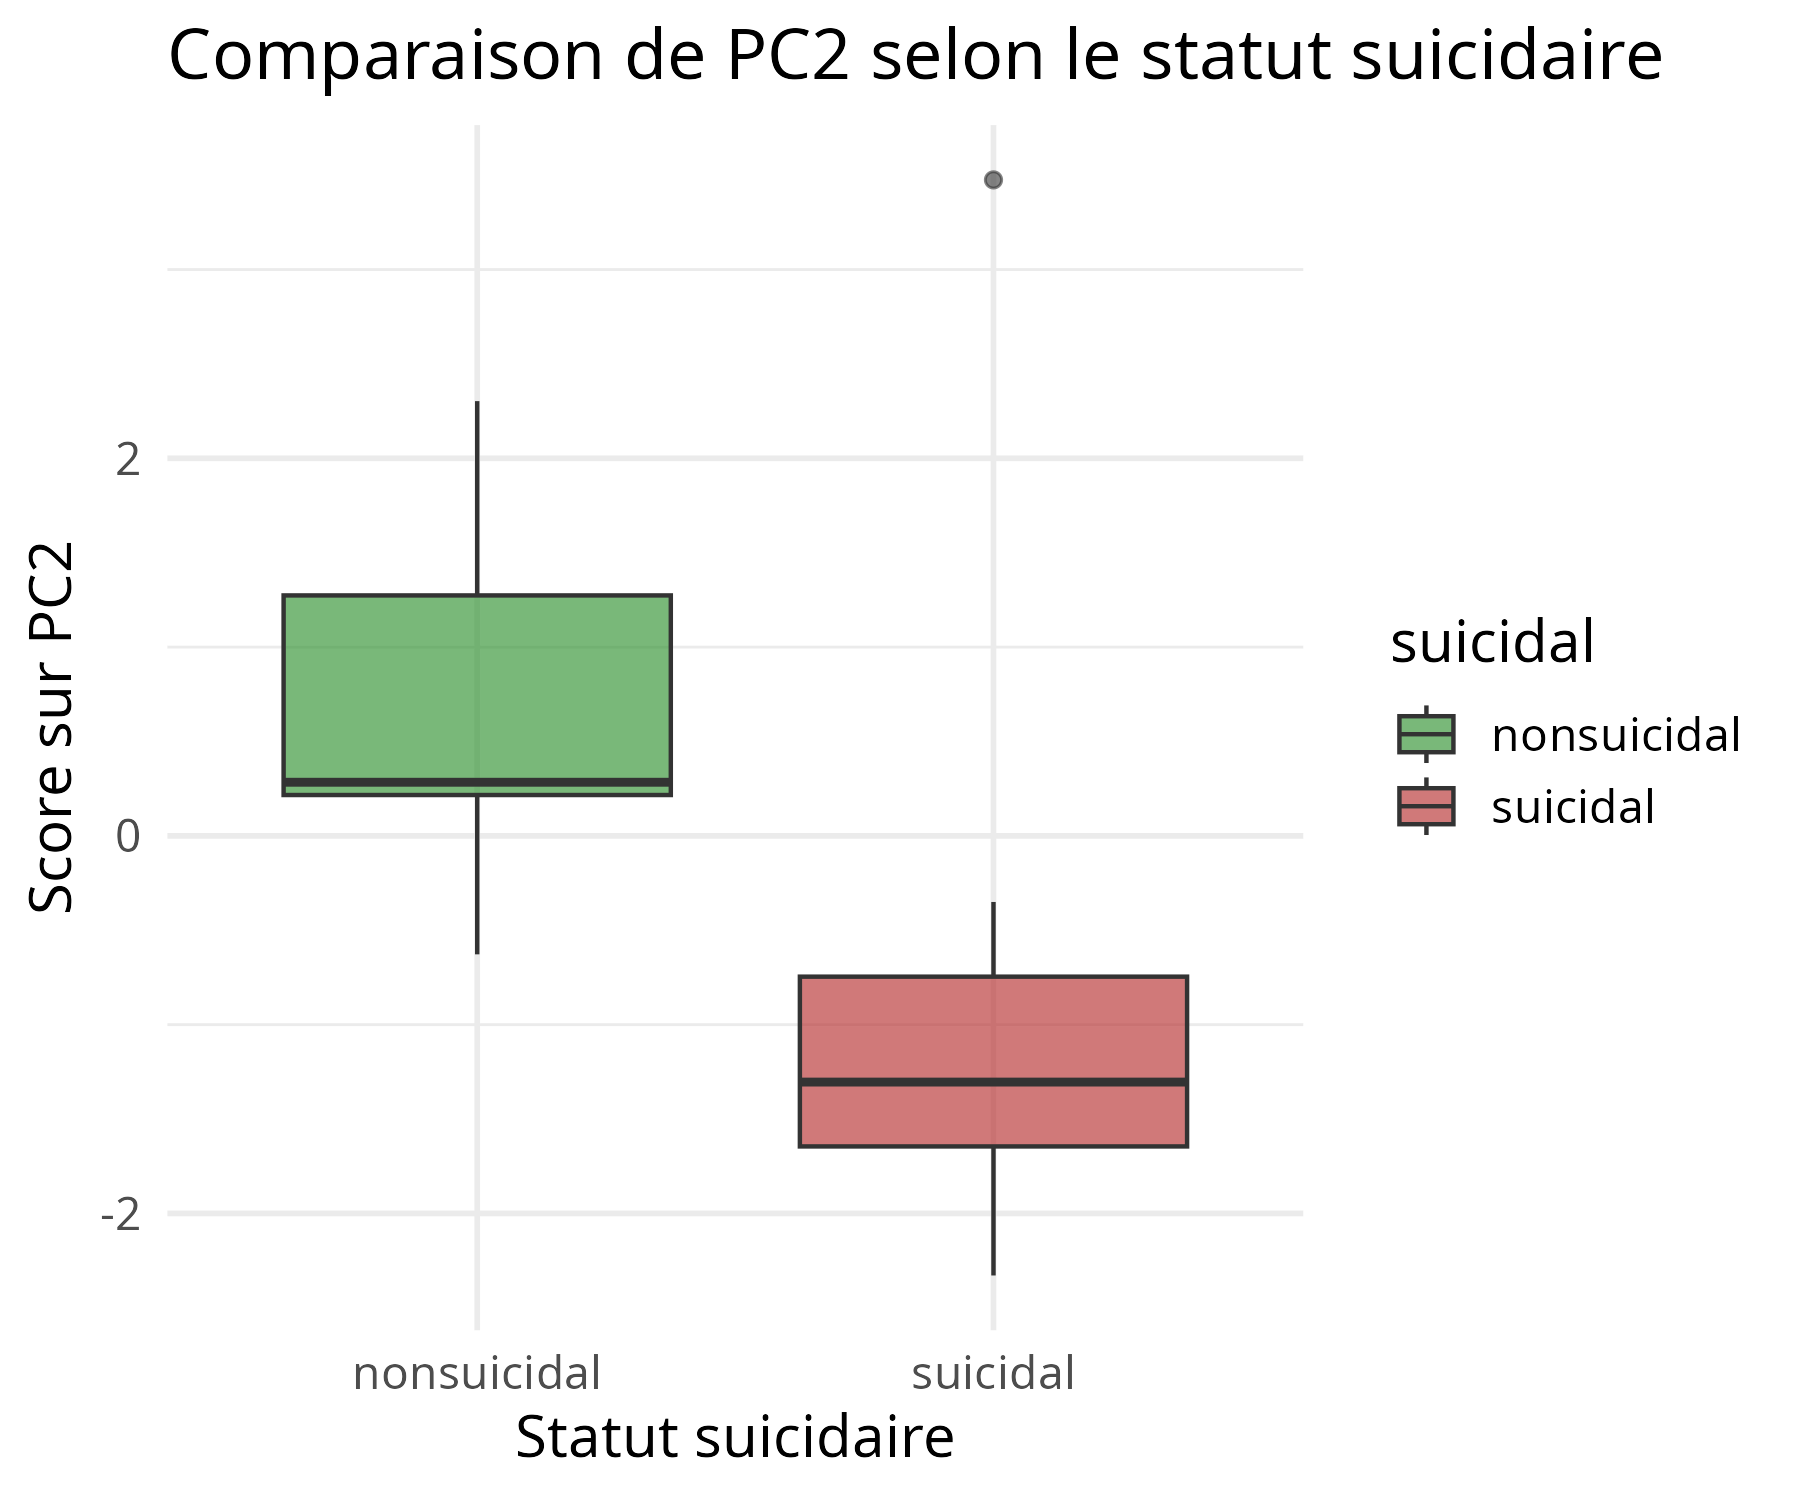
\includegraphics[width=0.49\textwidth]{06_boxplot_PC2.png}
	\caption{Boxplots comparant PC1 (gauche) et PC2 (droite) selon le statut suicidaire.}
	\label{fig:boxplots_pc1_pc2}
\end{figure}

Les boxplots (Figure~\ref{fig:boxplots_pc1_pc2}) montrent 
qu'aucun groupe ne se détache de façon flagrante. 
Afin d'étayer cela, on effectue un \textit{Welch Two Sample t-test} 
pour chacune des composantes (PC1 et PC2). 
Les résultats se trouvent dans le fichier \texttt{07\_tests\_statistiques.txt} 
et sont reproduits ci-dessous.

\paragraph{Test sur PC1.}
\begin{verbatim}
	t = 1.6581, df = 9.2921, p-value = 0.1306
	IC 95%: [-0.6681746, 4.4029684]
	Moyenne (nonsuicidal) = 0.9336984
	Moyenne (suicidal)    = -0.9336984
\end{verbatim}

\paragraph{Test sur PC2.}
\begin{verbatim}
	t = 1.7063, df = 9.0007, p-value = 0.1221
	IC 95%: [-0.4597469, 3.2824927]
	Moyenne (nonsuicidal) = 0.7056865
	Moyenne (suicidal)    = -0.7056865
\end{verbatim}

Dans les deux cas, la \textit{p-value} est supérieure à 0,05, 
indiquant qu'il n'y a pas de différence statistiquement significative 
entre poètes suicidaires et non suicidaires 
concernant les scores moyens sur PC1 ou PC2. 
On note cependant que les moyennes présentent des signes inverses 
(``positifs'' pour les poètes non suicidaires et ``négatifs'' pour les suicidaires). 
Ce ``renversement'' n’est pas suffisant pour être jugé significatif 
au vu de l’échantillon restreint (\textit{p-value} > 0,1). 

En conclusion, l’ACP permet de visualiser les différences (ou similarités) 
dans l’espace des émotions, mais elle ne révèle pas, selon ces tests, 
de séparation nette entre poètes suicidaires et non suicidaires 
sur les deux premières composantes.

%----------------------------------------------------------

	
	%============================================================
\end{document}
